\chapter{\LaTeX で図を用いるときのコツ} \label{apdx:tips}
Power Pointで図を作成してPNGやJPGなどで保存すると,デフォルトでは画像が粗くなる.
そこで,付録\ref{apdx:tips}ではPower Pointで作成した画像が
綺麗なまま\LaTeX で画像を表示させる方法を述べる.

以下,上記の手法の手順を示す.なお,以下のステップ$3$から$7$までの過程は図\ref{fig:method}に,
出力結果の例は\ref{fig:pdf}に示した.
\begin{enumerate}
    \item 予め,SVG画像を編集できるソフトをインストールし,使える状態にする
        (ここでは,Inkscapeというよく使われている無料ソフトを用いる~\cite{inkscape}).
    \item \LaTeX の編集ソフトとPower Point,Inkscapeの三つを開き,
        Inkscapeは新規ドキュメントを作成し待機する.
    \item Power Pointで保存したい図を選択し(グループ化しておくと確実),コピーする.
    \item コピーした画像を Inkscape の新規ドキュメントに貼り付ける.
    \item Inkscapeの「ファイル(F)」の「名前を付けて保存(A)...」を選択(ショートカットキーはWindowsなら「Ctrl+Shift+S」).
    \item 「ファイルの保存先を選択」というポップアップが現れるので,「ファイルの種類(T):」からPDFを選択して「保存(S)」をクリックする.
    \item 「Portable Document Format」というポップアップが現れ,図のように「テキスト出力オプション」を「フォント埋め込み」にし,「フィルターエフェクトをラスタライズする」の項目を外し,「出力ページサイズ」を「エクスポートオブジェクトのサイズを使用」に変更して「OK(O):」を選択する.
    \item 保存したPDFを確認すると,拡大しても画像が粗くないことが分かる.
    \item 画像を\LaTeX で参照すれば無事に図\ref{fig:pdf}のようになる.
    \item 次からの画像は,ステップ$3$から順に行なえば良い.
\end{enumerate}
ただし,ここで用いたInkspaceは$2023$年$11$月現在での最新版(Inkscape$1.2$)の場合であるため,
アップデートなどを経てUIが変わり分かりづらくなる可能性もある.

% === figure === %
\begin{figure}[h]
  \centering
  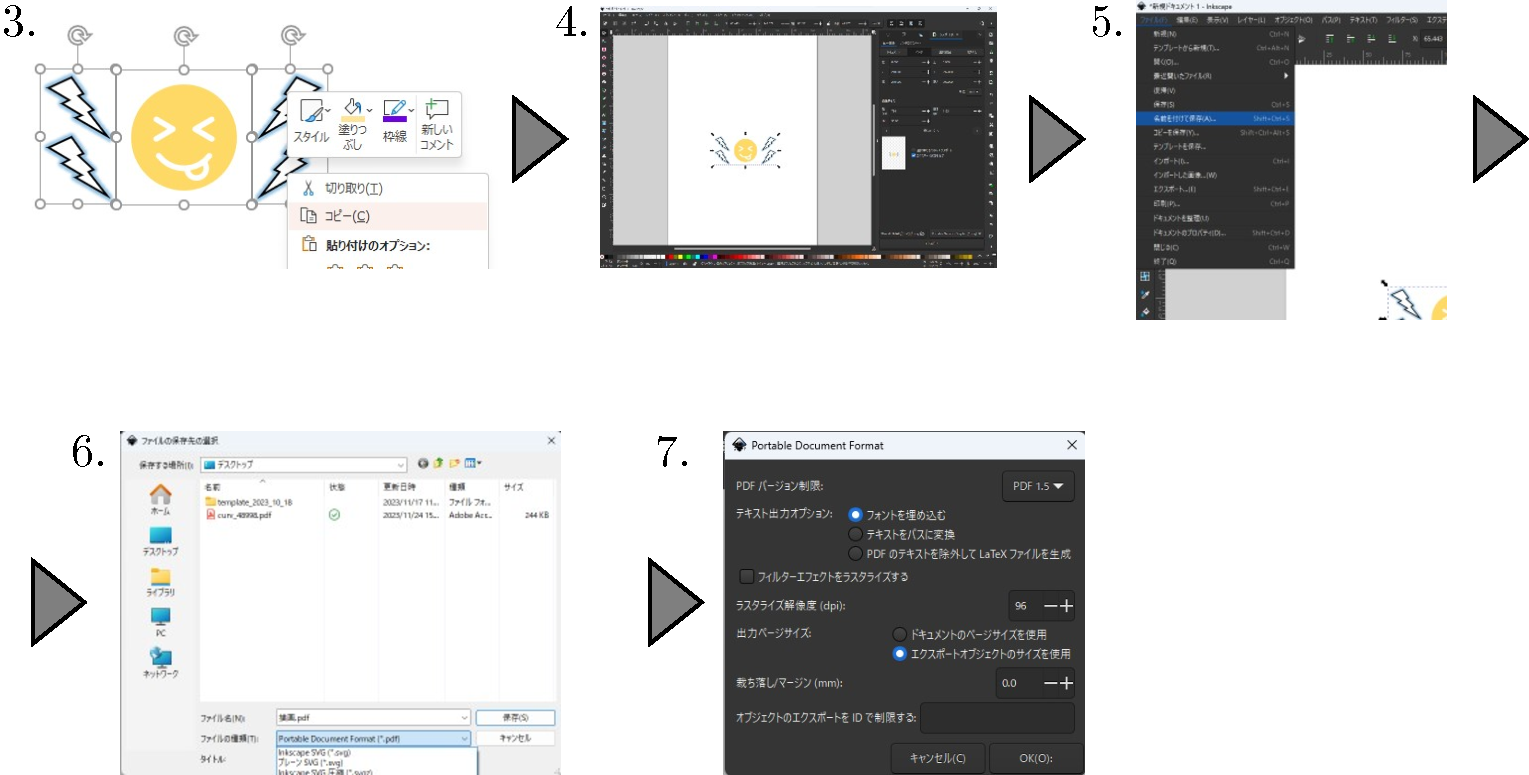
\includegraphics[keepaspectratio, width=0.9\linewidth]{method.pdf}
  \caption{ステップ$3$から$7$までの過程.
  スクリーンショットのため見づらいが拡大表示するなどして確認して欲しい.}
  \label{fig:method}
\end{figure}
% === figure === %
% === figure === %
\begin{figure}[h]
  \centering
  
\includegraphics[keepaspectratio, width=0.6\linewidth]{picture.pdf}
  \caption{作成したPDFファイル.拡大しても粗くならない.
  Cloud LaTeX上では日本語名PDFはエラーになったので,描画.pdf $\to$ picture.pdfに変更.}
  \label{fig:pdf}
\end{figure}
% === figure === %
